\section{Theory}

\begin{frame}{Hybrid ASR system \cite{RASR-hybrid_vs_attention}}

\begin{itemize}
    \item \textbf{Bayes theorem}: The relation $w^{*}$ between the acoustic observations $x_{1}^{T}$ whose length is $T$ and the most likely word sequence to be recognized $w_{1}^{N}$:
    \begin{equation}
    w^{*} = \operatorname{arg}\max_{w_1^N}  \underbrace{p(x_{1}^{T}|w_{1}^{N})}_{\text{acoustic model}}\cdot\underbrace{p(w_{1}^{N})}_{\text{language model}}
    \end{equation}
    
    \item \textbf{Gammatone feature extraction} \cite{schlueter:icassp07}:
    Hanning window \textrightarrow \, (10th root or log) compression \textrightarrow \, DCT-based cepstral decorrelation \textrightarrow \, normalization
    
    \item \textbf{Hidden Markov Model (HMM)}:
    \begin{align}
    	\label{eq:hmm}
    	p(x_1^T|w_1^N) = \sum_{[s_1^T]}\prod_{t=1}^Tp(x_t, s_t|s_{t-1}, w_1^N) =
    	\sum_{[s_1^T]}\prod_{t=1}^T\underbrace{p(s_t|s_{t-1}, w_1^N)}_{\text{transition prob.}}\cdot
    	\underbrace{p(x_t|s_t, s_{t-1}, w_1^N)}_{\text{emission prob.}}
    \end{align}

\end{itemize}

%\TODO{I suggest that you don't have full sentences on your sldies for two reasons: 1. audience will be occupied with reading and pay less attention to you 2. the danger might arise that you read from the slides and do not hold a talk but a reading}

\end{frame}

\begin{frame}{Hybrid ASR system \cite{RASR-hybrid_vs_attention}}

\begin{itemize}
    \item \textbf{Context-Dependent Phone}: generate triphone or allophone labels
    
    \item \textbf{CART} \cite{Beulen98automaticquestion}: To cluster triphones \textrightarrow \, reduce the number of labels
    
    \item \textbf{Baum–Welch algorithm}: To find the best alignment between acoustic observations and transcriptions:
        \begin{enumerate}
            \item Maximization
        	\item Expectation 
        	\item Get back to step 1 
        \end{enumerate}
        
\end{itemize}
\end{frame}

\begin{frame}{Hybrid ASR system \cite{RASR-hybrid_vs_attention}}

\begin{itemize}
    \item \textbf{GMM/HMM system}: HMM to model the transition between phones and the corresponding observable, GMM to model the emission probabilities
    %The GMM is a weighted sum over $K$ normal distributions:
    %\begin{align}
    %	p(x_t|s_t, s_{t-1}, w_1^N) = \sum_{i=1}^K c_i \cdot \mathcal{N}(x_t|\mu_i, \sigma_i^2),
    %\end{align}
    %\TODO{where did you get this formula from?}
    %resulting in a multimodal emission probability with parameters $\mu_i, \sigma_i$ and mixture weights $c_i$ for $i\in\llbracket1,K\rrbracket$.
    
    \item \textbf{DNN/HMM system}: DNN to model the posterior probability $p(a_{s_t}|x_t)$ discriminatively.
    The emission probability in the HMM can be calculated such that:
    \begin{align}
    	p(x_t|a_{s_t}) = \frac{p(a_{s_t}|x_t)p(x_t)}{p(a_{s_t})}.
    \end{align}
    The probability $p(a_{s_t})$ can be estimated as the relative frequency of $a_{s_t}$.
    The probability $p(x_t)$ can be removed.
\end{itemize}
\end{frame}

\begin{frame}{Hybrid ASR system \cite{RASR-hybrid_vs_attention}}
\begin{itemize}
    \item \textbf{Language modeling (LM)}: 4-gram count based LM, using Kneser-Ney Smoothing algorithm \cite{kneser_ney_lm}. 
    Full-words used in the first-pass decoding \cite{beck2019lstm}. 
    %\TODO{there is no 2nd pass decoding at all! make this more clear}
    
    \item \textbf{Decoding}: With the help of the Viterbi approximation:
    \begin{align}
    	w_1^N = \operatorname{arg}\max_{N,w_1^N}p\Bigl(\prod_{n=1}^Np(w_n|w_{n-m}^{n-1}) \cdot
    	\max_{[s_1^T]}\prod_{t=1}^Tp(x_t,s_t|s_{t-1}, w_1^N)\Bigr),
    \end{align}
    Beam search (AM and LM pruning) used to only focus on the most promising predicted words at each time step \cite{ortmanns1997word}.
    
    \item \textbf{Recognition performance}: The Word-Error-Rate (WER) indicator is used:
    \begin{equation}
        \text{WER} = \frac{\text{Substitutions} + \text{Insertions} + \text{Deletions}}{\text{Reference words}}
    \end{equation}

\end{itemize}
\end{frame}


\begin{frame}{wav2vec 2.0 \cite{facebookwav2vec2}}

\newcommand{\cSeq}{$\mathbf{c}_1^{T_{w2v}}$}
\newcommand{\qSeq}{$\mathbf{c}_1^{T_{w2v}}$}

\begin{itemize}
    \item \textbf{Self-supervised learning}:
\end{itemize}

\begin{figure}[hbtp]
    \centering
    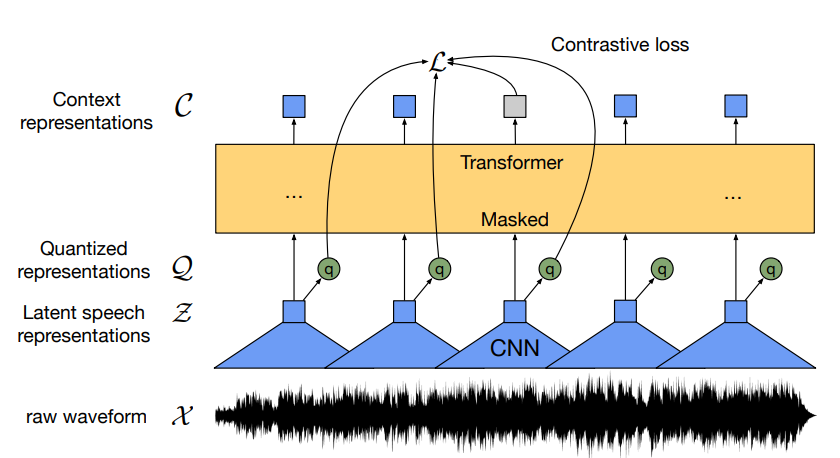
\includegraphics[width=0.7\textwidth]{figures/speech_representation_wav2vec2.PNG}
    \caption{\center{Illustration of wav2vec 2.0 framework which jointly learns contextualized speech representations
    \\and an inventory of discretized speech units.}}
    \label{speech_representation_wav2vec2}
    \end{figure}
    
\end{frame}


\begin{frame}{wav2vec 2.0 \cite{facebookwav2vec2}}

\begin{itemize}
    \item \textbf{Feature encoder}: Blocks of temporal convolution, layer normalization \cite{layer_normalization}, and the GELU activation function \cite{gelu}. 

    \item \textbf{Contextualized representations with Transformers}: A context network that uses the Transformer architecture \cite{Transformer}. 
    
    \item \textbf{Contrastive learning}: Get a context representation $c_t$ for a masked latent representation $z_t$ in order to guess the proper quantized representation $q_t$ among alternative quantized representations.

    \begin{figure}[hbtp]
    \centering
    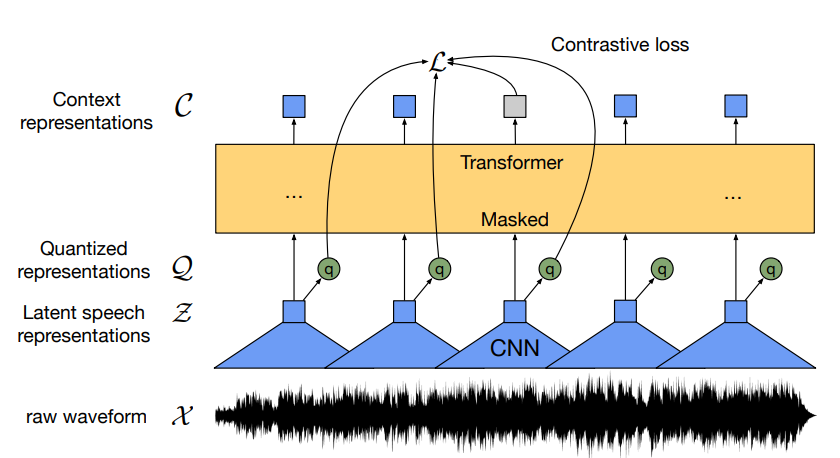
\includegraphics[width=0.5\textwidth]{figures/speech_representation_wav2vec2.PNG}
    \end{figure}
    
\end{itemize}

\end{frame}

% XLSR
\begin{frame}{Unsupervised cross-lingual representation learning (XLSR) \cite{XLSR}}

\begin{itemize}
    \item \textbf{XLSR}: By extending wav2vec 2.0 to the multilingual setting, cross-lingual learning seeks to create models that use data from other languages to improve performance. 
    
    \item \textbf{In-domain Match Level}:
     Determined by the similarity between recording conditions, naturalness and conversational topics.
    
    \item \textbf{Diversity Level}: of the multilingual dataset is higher than the monolingual one because the first represents more learnable phonemes helpful to target language.
\end{itemize}

\begin{figure}
    \centering
    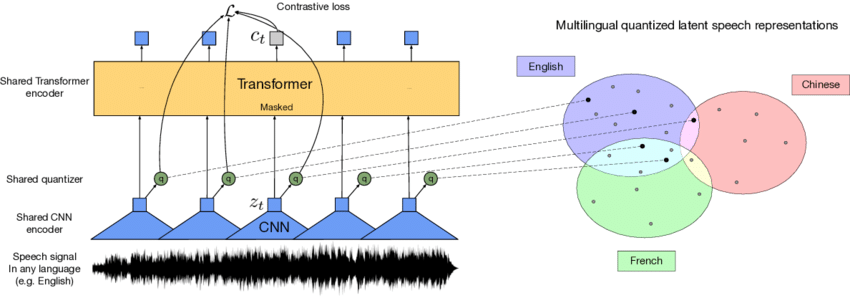
\includegraphics[width=0.8\textwidth]{xlsr_speech_representations.png}
\end{figure}
        
\end{frame}
